\documentclass[conference,letterpaper]{IEEEtran}
\usepackage[T1]{fontenc}
\usepackage{cite,amsmath,graphicx,listings,xurl}
\usepackage[hidelinks]{hyperref}
\interdisplaylinepenalty=2500
\lstset{basicstyle=\ttfamily\footnotesize,columns=fullflexible,keepspaces=true,
  breaklines=true,showstringspaces=false,frame=single,framerule=0.25pt,
  xleftmargin=3pt,xrightmargin=3pt,aboveskip=5pt,belowskip=5pt,
  keywordstyle=\bfseries,morekeywords={if,else,for,while,return,on,require,atomic,then}}
\newcommand{\code}[1]{\texttt{#1}}
\newcommand{\checkcase}[1]{\noindent\textit{Verification:} #1\par}
\title{Encore Moment\\[0.3em]
{\large PC-Based Audience Reaction Capture}\\[0.4em]
{\normalsize Group Encore}}
\author{
\IEEEauthorblockN{Chul Park}
\IEEEauthorblockA{Department of\\Information Systems\\
Hanyang University\\Seoul, Republic of Korea\\parkchul1@hanyang.ac.kr}
\and
\IEEEauthorblockN{Pavel Kim}
\IEEEauthorblockA{Department of\\Information Systems\\
Hanyang University\\Seoul, Republic of Korea\\skydish@hanyang.ac.kr}
\and
\IEEEauthorblockN{Soyeon Seol}
\IEEEauthorblockA{Department of\\Information Systems\\
Hanyang University\\Seoul, Republic of Korea\\ssy050915@hanyang.ac.kr}
\and
\IEEEauthorblockN{Yujeong Heo}
\IEEEauthorblockA{Department of\\Information Systems\\
Hanyang University\\Seoul, Republic of Korea\\gjdbwjd03@hanyang.ac.kr}}
\hypersetup{pdftitle={Encore Moment - Submission B: Specification},
pdfauthor={Group Encore},pdfsubject={CSE406 Software Engineering - Submission B}}
\begin{document}
\maketitle
\begin{abstract}
Encore Moment captures audience reactions as reviewable viewing memories. It is implemented as a PC application connected to a team-controlled test player and an AWS inference server. Playback-reference echo cancellation supplies audience audio for laughter, scream, and gasp recognition. Server-side audio and facial analysis produce events with observable intensity, content title, and playback timecode. An explicitly enabled camera feeds a local disk-based rolling buffer, from which variable-length audience clips are saved with available context and editing handles. A live timeline and Tonight's Highlights support review and deletion. This specification preserves thirteen requirements, defines the development environment and estimated cost, and gives an implementation procedure and verification case for each requirement. It also defines an iterative development process and a Kubernetes-deployable server package. These procedures describe planned behavior, not completed implementation or measured model performance.
\end{abstract}
\begin{IEEEkeywords}
audience reactions, acoustic echo cancellation, PC application, server inference, software specification
\end{IEEEkeywords}
\section{Introduction}
\subsection{Motivation}
A memorable viewing experience includes the people in the room. Friends may laugh at the same unexpected line, a couple may gasp at a plot twist, or a home party may erupt during a tense scene. These reactions happen without warning. Reaching for a phone after the moment has passed cannot recover the initial reaction, while recording an entire evening leaves users with material to search and edit.

Encore Moment helps viewers preserve these spontaneous moments while remaining engaged with one another and the screen. Friends, couples, families, and party guests may want to revisit a shared response without assigning someone to operate a camera. Streamers and reaction-content creators also need to find spontaneous reactions without reviewing an entire recording. The system identifies candidate moments and describes observable reactions rather than claiming to infer private emotions. Users decide whether a saved moment is suitable to keep or use elsewhere.

\subsection{User and Client Needs}
Viewers need relevant highlights, enough context to remember the scene, and controls that are easy to understand during viewing. A film's laugh track or scream should not be mistaken for a person in the room. Users should know when sensing is active, be able to stop it, and review or delete saved clips. Reaction intensity can help prioritize review, but it cannot determine a person's emotional state or the personal importance of a memory.

The client needs a PC application with a clear feature scope, understandable privacy controls, and explicit support for the demonstration devices and team-controlled player. The application must make sensing status, available highlights, and clip deletion easy to understand.

The demonstration uses a PC, a microphone, an optional webcam, and a player controlled by the team. The player supplies its decoded playback audio, title, position, and play/pause/seek changes. This makes acoustic echo cancellation (AEC) and scene association implementable without assuming access to third-party streaming applications. Saved video depicts the audience. Native TV integration, mobile clients, and recording the viewed program are outside this implementation baseline.

The PC preprocesses audio, manages sensing controls and a disk-based circular video buffer, and creates saved clips. The AWS server performs audio recognition, facial analysis, event fusion, and event-record management. High-quality audience footage stays on the PC; only analysis audio and reduced-resolution camera frames are transmitted. Saved audience clips are stored locally on the PC. Figure~\ref{fig:processing} summarizes this processing boundary. Section~III identifies development baselines that still require integration validation.

\begin{figure*}[!t]
\centering
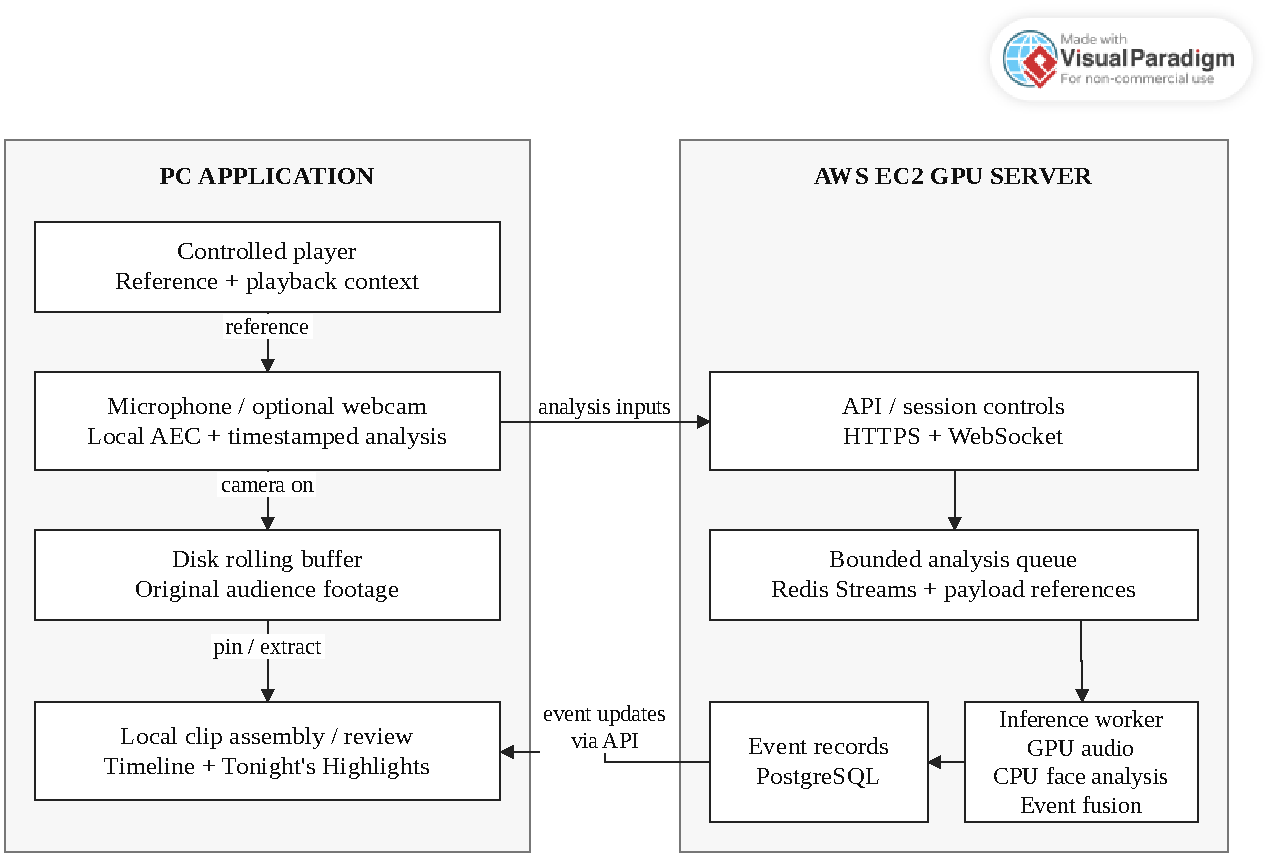
\includegraphics[width=0.88\textwidth]{images/processing-structure.pdf}
\caption{Planned processing structure. The controlled player supplies playback context as well as the AEC reference. Event updates return through the API; continuous original audience footage remains on the PC. Camera-dependent paths are inactive while the camera is off.}
\label{fig:processing}
\end{figure*}

\subsection{Related Software}
\textit{Capture and highlight services.} Reaction-triggered clipping is established in gaming and streaming software. SteelSeries Moments clips laughter and excited vocal reactions detected by the microphone, a feature later named Reaction Clipping~\cite{steel55,steel70}. Twitch Auto Clips creates clips through speech recognition and AI in an invitation-only alpha~\cite{twitch}, and Medal triggers clips from game events~\cite{medal}. OBS Studio exposes replay-buffer operations that illustrate retaining recent media and saving it on demand~\cite{obs}. Encore Moment adds reaction-driven selection, playback context, and sensing controls for shared viewing, where audience reactions must be separated from playback sound.

\textit{Sound event models.} The system will use a pretrained sound-event model such as YAMNet~\cite{yamnet} or PANNs~\cite{panns,pannsweights}. Both are trained on AudioSet, and their labels include laughter, screaming, and gasp. EfficientAT, BEATs, and CLAP remain secondary comparisons for resource use, pretrained representations, and zero-shot audio-text matching~\cite{efficientat,beats,clap}. Speech-emotion models such as audEERING's dimensional model predict arousal, dominance, and valence from podcast speech~\cite{audeering}; that task differs from brief nonverbal reactions, so classifier confidence, acoustic intensity, and emotional significance are kept distinct.

\textit{Facial observations.} MediaPipe Face Landmarker supplies facial landmarks and blendshape observations~\cite{mediapipe}. These can support reaction evidence but do not establish an emotional state or speaker identity.

\textit{Datasets.} FSD50K provides human-labeled laughter, scream, and gasp audio, but its clip-level labels give no precise reaction boundaries or intensity, and individual sound licenses must be checked~\cite{fsd50k}. FSDKaggle2019 has no laughter class and largely overlaps FSD50K~\cite{fsdkaggle,dcase}, so the two are not treated as independent training and evaluation sets. VocalSound adds confusable human sounds such as sighs and coughs but lacks gasp and scream~\cite{vocalsound}. Public data supports initial comparison; consented soundtrack-only, audience-only, and mixed room recordings are still required.

\textit{Echo cancellation and recording.} WebRTC's Audio Processing Module provides playback-reference and microphone interfaces for AEC~\cite{webrtc}, and the Microsoft AEC Challenge supplies data and baselines~\cite{aecchallenge}. Their use in speech applications does not show that nonverbal reactions survive cancellation. GStreamer's WebRTC audio-processing wrapper and segmented recording element provide the initial media building blocks~\cite{gst-aec,gst-ring}. NVIDIA DeepStream Smart Video Record likewise records from cached media before an event, with keyframe-related limits on the clip beginning~\cite{deepstream}.

\textit{TV interfaces.} LG Smart Cam provides camera and microphone hardware for LG TVs~\cite{lgcam}, but public webOS interfaces do not give ordinary applications access to its camera media or to raw playback audio~\cite{lgforum,lgaudio}. Encore Moment is therefore built as a PC application with a team-controlled player.

These sources do not demonstrate the performance of the proposed combined system in our viewing environment.

\subsection{Team Responsibilities and Roles}
Table~\ref{tab:roles} assigns development roles and module ownership; SW denotes software. Soyeon Seol additionally represents the course User role, and Pavel Kim the Customer role. These internal stakeholder roles support review of user and client needs. All members participate in requirement reviews and integration checks.

\begin{table}[!ht]
\caption{Module Ownership and Role Assignments}
\label{tab:roles}
\centering
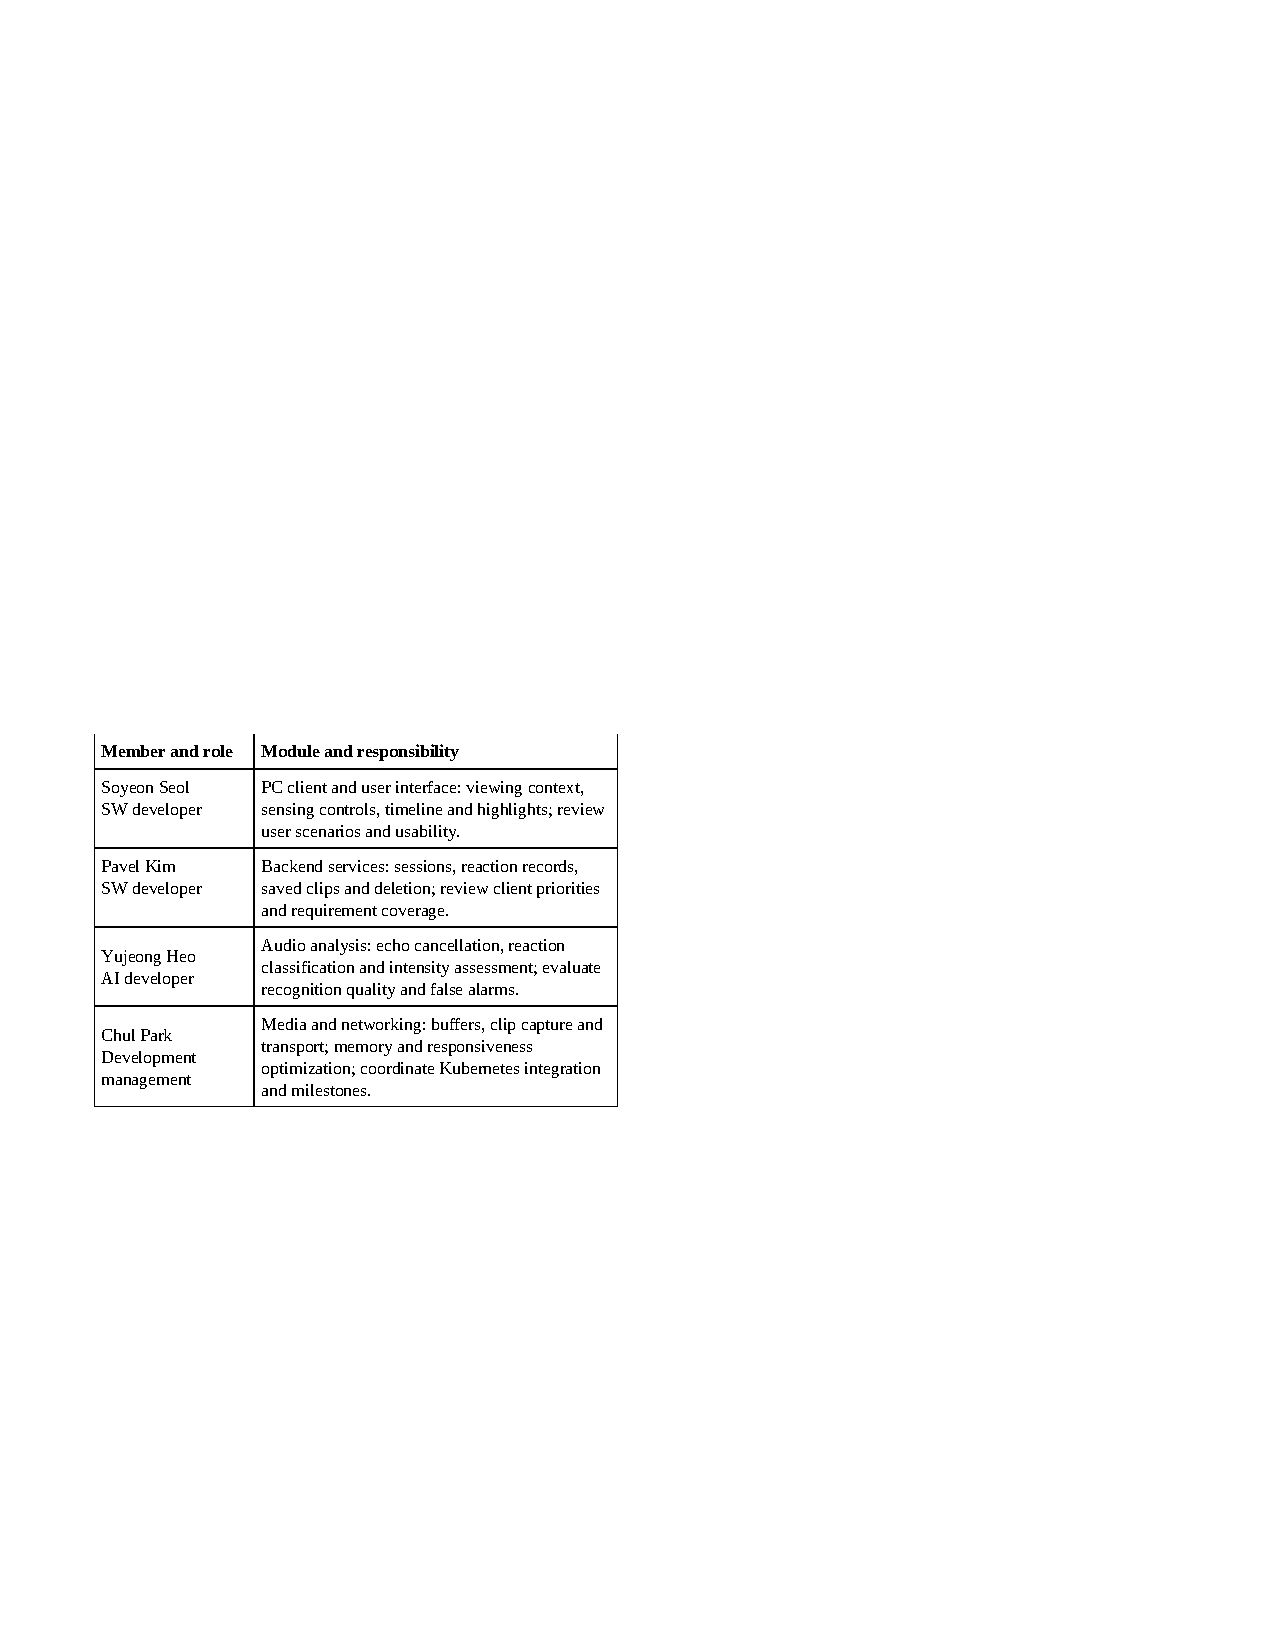
\includegraphics[width=\columnwidth]{images/team-roles.pdf}
\end{table}

This is Submission B, the specification stage of the course project~\cite{assignment}. The repository is \url{https://github.com/SWE-encore/encoremoment}. This document's sources are maintained in \code{submission-b/}. Section~III-C describes the development process and integration responsibilities.

\section{Requirements}
Saved video means audience footage. The following thirteen requirements define the viewing workflow and server deployment, with corresponding specifications in Section~IV. They are divided by development priority: must-have requirements form the core viewing workflow and sensing controls and are developed first, and good-to-have requirements are developed after the must-have set works end to end.

\subsection{Must-Have Requirements}
\noindent\textit{Requirement 1: Echo Cancellation:} The system shall use the playback reference to suppress playback sound in microphone audio while retaining audience sound for reaction analysis.

\noindent\textit{Requirement 2: Reaction Recognition:} The system shall classify detected audience sounds into at least laughter, scream, and gasp.

\noindent\textit{Requirement 3: Event Records:} The system shall record each detected reaction with its type, observed intensity, content title, and timecode. Intensity shall describe the observable reaction rather than an inferred internal emotion.

\noindent\textit{Requirement 4: Highlights:} After viewing, the system shall present Tonight's Highlights, prioritizing high-intensity reaction segments and linking any available audience clips for user review.

\noindent\textit{Requirement 5: Camera Activation:} The camera shall be off by default and activated only by explicit user action. No video shall be captured, buffered, or uploaded while it is off.

\noindent\textit{Requirement 6: Camera Indication:} The interface shall show a persistent indicator while the camera is active and provide a control to stop capture.

\noindent\textit{Requirement 7: Review and Deletion:} Users shall be able to review and delete saved reaction clips and their associated media at any time. The interface shall indicate whether a deletion request is pending or completed.

\noindent\textit{Requirement 8: Microphone Control:} Users shall be able to disable microphone-based sensing. This shall stop audio capture, upload, and new audio-triggered detections, with the disabled state shown clearly.

\noindent\textit{Requirement 9: Viewing Interface:} The interface shall display a real-time reaction timeline, the highlight list, and the current sensing and connection status.

\noindent\textit{Requirement 10: Reaction Clips:} With the camera enabled, the system shall save an audience clip for each detected reaction, starting 15~s before and ending 10~s after the trigger. Each time the detection threshold is exceeded again before the clip ends, the clip end shall be extended by 5~s, up to a maximum clip length of 60~s. Missing portions shall be indicated; no footage from before camera activation shall be assumed to exist.

\noindent\textit{Requirement 11: Viewing Sessions:} Users shall be able to start and end sensing sessions. The system shall report connection interruptions, avoid duplicate reaction records after reconnection, and clear unsaved temporary media when a session ends.


\subsection{Good-to-Have Requirements}
The server-side processing in Requirement 13 is already used by the must-have pipeline through Docker Compose; its Kubernetes deployability is the part developed later.

\noindent\textit{Requirement 12: AEC Control:} The system shall provide an option to turn echo cancellation on and off and show the selected mode.

\noindent\textit{Requirement 13: Server Deployment:} The team shall provide server-based AI and computational processing, with the server components deployable on Kubernetes, a platform for managing containerized workloads and services~\cite{kubernetes}.


\section{Development Environment}
\subsection{Platform, Languages, and Cost}
\subsubsection{PC and server platforms}
Linux is the first client target because it offers direct camera/microphone access and a common GStreamer pipeline for controlled playback and capture. Python is selected for application logic and server inference; PySide6 provides the desktop interface, and PyGObject connects the client to GStreamer. Asynchronous acquisition and inference prevent a slow network or model from blocking sensor controls. The reproducible client target is Ubuntu 24.04 LTS, Python 3.12, PySide6 6.8.3, GStreamer 1.24, and FFmpeg 6.1. These are selected integration baselines, not a claim that the application already runs on them.

The inspected workstation runs Ubuntu 26.04.1 LTS on an AMD Ryzen AI 7 350 with 8 cores/16 threads and approximately 14.2~GiB of OS-visible RAM. The client will be tested in its specified environment before distribution; host-installed packages are not the dependency lock. Webcam and microphone models will be recorded during the capture trial. The plan assumes existing equipment, not a new PC or GPU purchase.

The AWS target is one Linux \code{g4dn.xlarge} in Asia Pacific (Seoul): 4 vCPUs, 16~GiB RAM, and one NVIDIA T4 with 16~GiB GPU memory~\cite{ec2spec}. An 80~GB encrypted gp3 EBS volume holds the database, model files, and bounded temporary analysis data. Durable records do not depend on instance-store survival. Docker Compose runs the API, queue, database, and inference services on this host. One resident audio model uses the GPU; facial analysis initially uses CPU within the inference service. This preserves server-side audio and video analysis without duplicating GPU model allocations. Load measurements will determine whether concurrency or instance size must change.

\subsubsection{Software baseline}
The server target is Ubuntu 24.04 LTS with separate Python 3.11 environments for the API and inference worker. Proposed pins are FastAPI 0.162.0, PyTorch 2.9.1 with CUDA 12.6, MediaPipe 0.10.21, and NumPy 1.26.4 in the worker. Redis 7.2 provides a bounded work stream; PostgreSQL 16 stores sessions, events, result cursors, and deletion state. Docker Engine 28 and Compose 2 are the server packaging baseline. Exact patch versions, image digests, compatible NVIDIA driver/container-toolkit versions, model checksums, and the PANNs source revision will be locked after clean installation and an end-to-end inference trial. A dependency lock alone does not prove model or media compatibility.

\subsubsection{Estimated expenditure}
The estimate uses Linux shared-tenancy On-Demand pricing in Seoul, checked November 4, 2026: \$0.647 per GPU-instance hour, \$0.0912 per GB-month of gp3 storage, and \$0.005 per public IPv4 address-hour~\cite{ec2price,ipv4}. For 80~GB-month of EBS and one retained IPv4 address for 720 hours,
\begin{equation}
 C(h)=0.647h+80(0.0912)+720(0.005).
\end{equation}
Thus 40, 80, and 120 active GPU hours cost \$36.78, \$62.66, and \$88.54, respectively, before credits and tax. EBS and an allocated public address can incur charges while the instance is stopped. This excludes paid data transfer beyond applicable allowances, extra storage, paid monitoring, and subsequently purchased devices or licenses.

Existing equipment is budgeted at \$0 incremental hardware cost. No paid development-tool subscription or model-training service is planned. Distribution must retain applicable software and model-license notices; PANNs code and pretrained weights have distinct licenses~\cite{panns,pannsweights}. No managed Kubernetes control-plane charge is included. New-account Free Tier credits are intended to offset eligible usage; actual account plan, remaining credit, GPU quota, and expiry are unverified. GPU capability remains in the design even if eligibility requires another funding arrangement~\cite{freetier}.

\begin{table*}[!t]
\caption{Selected Development Baseline (Integration Validation Pending)}
\label{tab:baseline}
\centering
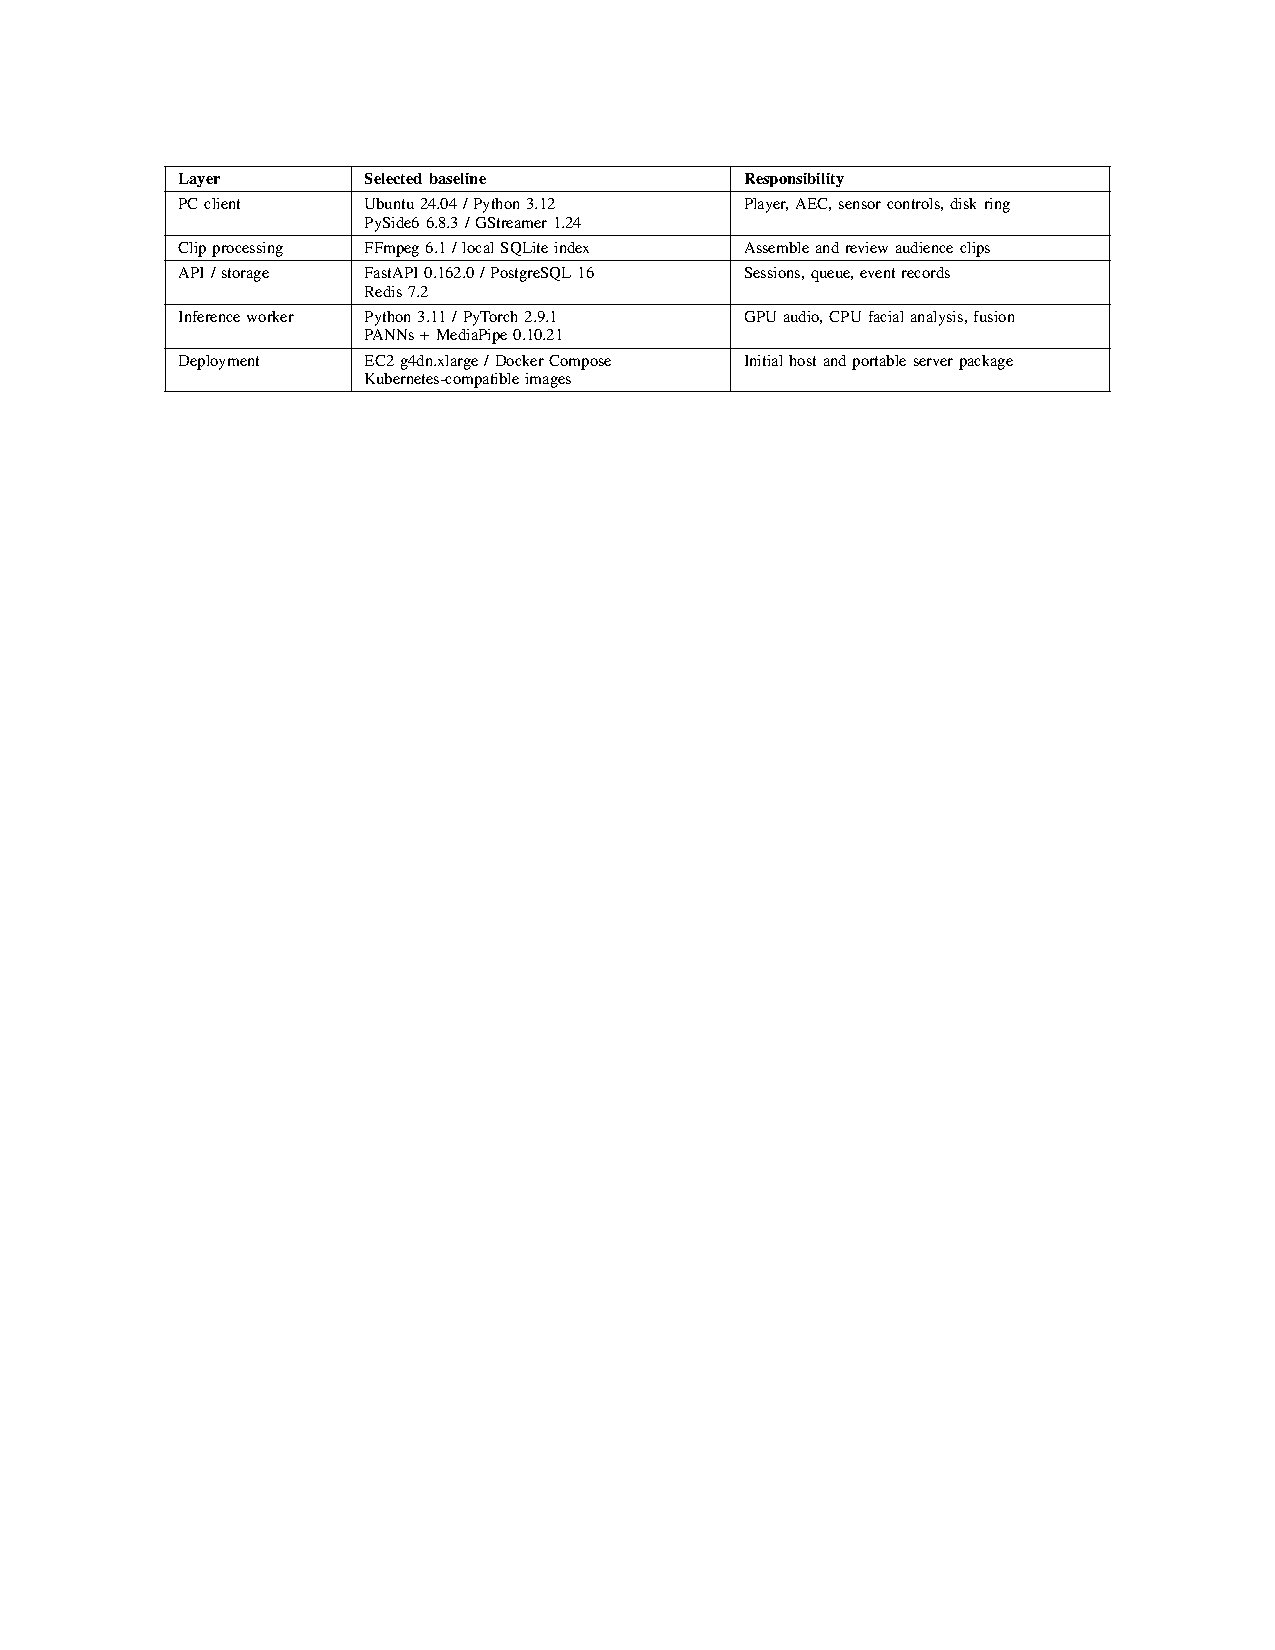
\includegraphics[width=\textwidth]{images/development-baseline.pdf}
\end{table*}

\subsection{Software and Processing Choices}
Table~\ref{tab:baseline} summarizes the selected layers and responsibilities.
GStreamer routes decoded player PCM through \code{webrtcechoprobe} before speaker output, while \code{webrtcdsp} processes microphone input in the same top-level pipeline. The probe is created before the DSP input becomes active; both branches use the same sample rate~\cite{gst-aec}. This is local signal preprocessing; reaction inference remains on the server. Camera video is split into independently decodable segments for the disk buffer. A reduced-resolution branch supplies analysis frames. FFmpeg assembles selected local segments into a reviewable clip, without uploading continuous original footage.

The initial audio candidate is PANNs \code{Cnn14\_DecisionLevelMax}, its pretrained AudioSet checkpoint, and 32~kHz mono input~\cite{panns,pannsweights}. Time-resolved output is mapped to capture timestamps. ``Screaming,'' ``Laughter,'' and ``Gasp'' map to the required classes. MediaPipe supplies per-face observations~\cite{mediapipe}; track identifiers are session-local and do not identify people. A single room microphone does not establish speaker-to-face identity. Classification confidence, observable intensity, and facial evidence remain distinct quantities.

The API accepts timestamped packets and places references to bounded temporary payloads into Redis Streams. Workers acknowledge jobs after event/result transactions commit. Stable keys make retries idempotent; at-least-once delivery is not exactly-once inference~\cite{redis}. The PC stores its clip index and result cursor in SQLite; PostgreSQL stores server event state. Saved clips remain local in this baseline. Server payloads expire after processing or a bounded retention interval; expiry produces an explicit dropped-input status.

\subsection{Responsibilities and Iterative Process}
The existing roles are retained. Soyeon Seol develops the PC interface and represents the User role; Pavel Kim develops backend/session/record services and represents the Customer role; Yujeong Heo develops AEC integration, audio recognition, and intensity evaluation; Chul Park manages development, media buffering/transport, and deployment integration. Facial-analysis integration is planned with AI/media work and needs a named issue owner before implementation. All members review requirement coverage and integration.

GitHub Issues and Projects will manage work beside source and pull requests~\cite{projects}. The proposed process uses one-week timeboxes, relative estimates, and capacity agreed at planning. This cadence is a project choice, not a lecture-mandated duration. Each issue identifies a Requirement number, acceptance case, owner, reviewer, estimate, and iteration. Board states are Backlog, Ready, In Progress, Review, and Done. Each developer begins with one active implementation task; blocked work is discussed before taking another.

At a brief daily check-in, members report completed work, today's work, blockers, omissions, and useful learning; problem solving follows separately. This follows the lectures' story/task planning, stand-up questions, and continuous integration guidance~\cite{lifecycle,management}. Weekly demonstrations with the User and Customer representatives drive reprioritization, followed by a short retrospective. Unfinished work returns to planning. Requirement changes require explicit review rather than silent removal to fit a sprint.

The first increment connects player reference, PC capture, server recognition, and a returned event. Later increments add clips/review, then failure handling and deployment checks. Good-to-have requirements are scheduled only after every must-have requirement passes its acceptance case. Integration and documentation target the recorded December 3, 2026 development milestone. Weekly scope follows demonstrated capacity. A task is Done when its acceptance case passes, a teammate reviews it, and the merged build works. CI will run unit/contract tests, supported media-fixture tests, container builds, and LaTeX compilation. Hardware/GPU checks run on the corresponding device, with evidence linked to the issue. Expected outcomes for AI-generated code are reviewed independently of that code.

\section{Specifications}
All procedures below describe the implementation to be built. The shared packet header contains \code{session\_id}, sensor/control generation, sequence number, capture timestamp, format, and playback epoch. A generation changes when a sensor is disabled/re-enabled; a playback epoch changes on seek or content change. Event IDs remain stable across updates and retries. State-changing requests carry an idempotency key. Invalid or expired inputs return an explicit status rather than silently producing a successful result.

\subsection{Requirement 1: Echo Cancellation}
\textit{Input/output:} microphone PCM and the controlled player's playback reference produce cleaned audience PCM and an AEC status. Both streams use 48~kHz during AEC; output is resampled to the audio model's 32~kHz input. Playback/capture timestamps use the PC's monotonic clock. The playback probe and microphone DSP share one top-level GStreamer pipeline, with the probe initialized first~\cite{gst-aec}.
\par\smallskip\noindent\begin{minipage}{\columnwidth}
\begin{lstlisting}
on microphone_block(m, capture_time):
  if microphone_disabled: return
  ref = playback_reference_for(capture_time)
  if AEC_requested and ref.valid:
    y = echo_cancel(m, ref)
    status = ACTIVE
  else:
    y = m
    status = reference_status(AEC_requested)
  enqueue_analysis(resample(y, 32000), status)
\end{lstlisting}
\end{minipage}\par
Playback seek, device change, or timing discontinuity resets alignment and marks AEC as warming up. If the reference is unavailable, the interface reports this and marks uncancelled input; it does not claim echo removal. Automatic gain control and additional noise suppression are disabled in the initial AEC trial to avoid concealing changes in nonverbal reaction strength. Their later use requires preservation checks. Saved audience footage uses the permitted captured microphone track, not the program's reference audio.
\checkcase{Compare AEC-on/off with soundtrack-only, audience-only, and overlapping playback/reaction recordings. Inspect residual playback and whether laughter, scream, and gasp remain recognizable; include seeks and output-device changes.}

\subsection{Requirement 2: Reaction Recognition}
\textit{Input/output:} timestamped cleaned audio and, when enabled, camera frames produce labeled reaction intervals. The GPU worker loads PANNs once and runs overlapping audio windows. Window length, stride, thresholds, and model checksum are versioned configuration. Framewise predictions are approximate temporal evidence, not exact acoustic onset measurements~\cite{panns}.

The initial fusion rule uses high-confidence audio alone, or a lower audio threshold supported by a strong valid facial reaction. For each sound class $c$, $p_c$ is model confidence, $I_a$ is normalized audio strength, and $V=\max_i v_i$ is the maximum valid per-face reaction score. Multiple weak faces do not accumulate into a strong response. A strong reaction from one person can therefore contribute without requiring a group average. No camera or missing faces means audio-only operation, not a failed session. Facial evidence never relabels a gasp as a sigh or substitutes an inferred emotion for a required sound class.
\par\smallskip\noindent\begin{minipage}{\columnwidth}
\begin{lstlisting}
for each aligned analysis_window w:
  if stale_generation(w): discard(w); continue
  p = audio_model(w.audio)
  c = best_of(p, [laughter, scream, gasp])
  V = max_valid_face_score(w.frames, default=0)
  strong = p[c] >= high[c] and Ia(w) >= min_audio
  supported = p[c] >= low[c] and V >= visual_gate
  accepted = strong or supported
  event = update_interval(c, accepted, hysteresis)
  emit_if_changed(event.OPEN, UPDATE, or FINAL)
\end{lstlisting}
\end{minipage}\par
Facial observations use normalized landmark/blendshape changes with pose, visibility, and tracking-validity checks; they do not identify a person's internal state. Open/close hysteresis and a gap tolerance merge adjacent windows of the same class. Different classes remain distinguishable. Ordinary speech, background noise, and uncertainty must pass the same evidence gates rather than automatically becoming an event. Thresholds are calibrated on development recordings and evaluated on separate recordings; no accuracy percentage is asserted here.
\checkcase{Use labeled laughter/scream/gasp, speech, soundtrack-only, and mixed recordings. Test camera-off operation, missing/occluded faces, one strong person, and several weak responses. Report per-class errors and measured detection delay.}

\subsection{Requirement 3: Event Records}
\textit{Input/output:} an accepted interval and playback anchors produce an upserted event with type, observed intensity, title, and content timecode. Each player anchor records capture time $t_0$, playback position $p_0$, playback rate $r$, play state, and content identity. Within a continuous playing epoch, timecode is $p(t)=p_0+r(t-t_0)$; pause keeps position fixed. An event crossing a seek/content boundary is split by epoch. Network arrival time never substitutes for capture time.

Audio intensity $I_a$ is the cleaned-audio RMS level relative to the calibrated room baseline, clipped to a configured range. Visual intensity uses the largest valid per-face observation $V$. The working combined intensity is $I=\max(I_a,V)$ after per-modality normalization. Stored fields retain both values and modality availability; confidence is not used as intensity. This is a ranking signal within a viewing session, not a calibrated physical loudness or emotional score.
\par\smallskip\noindent\begin{minipage}{\columnwidth}
\begin{lstlisting}
on event_update(e):
  anchor = get_anchor(e.start, e.epoch)
  if anchor missing: hold_pending(e); return
  record = {e.id, e.type, observed_intensity(e),
            anchor.title, map_time(e, anchor)}
  atomic:
    require current(e) and not deleted(e.id)
    upsert_event(record, key=(session_id, e.id))
    append_result_change(record)
  acknowledge_job()
\end{lstlisting}
\end{minipage}\par
Additional implementation fields include capture start/end, model/configuration version, AEC mode, event revision, and clip availability. Missing playback context is visible as pending and is retried; it is not fabricated. The controlled-player handshake supplies title and anchors before normal sensing begins.
\checkcase{Replay the same input/result twice and obtain one event. Check timecodes before/after pause, seek, rate change, and title change, including delayed network delivery.}

\subsection{Requirement 4: Highlights}
\textit{Input/output:} a session's committed event records and local clip index produce Tonight's Highlights. Finalized events are sorted by descending observed intensity, with capture time and event ID as deterministic tie-breakers. Events without footage remain reviewable as metadata. Overlapping events may point to one clip without losing their separate event records.
\par\smallskip\noindent\begin{minipage}{\columnwidth}
\begin{lstlisting}
on show_highlights(session):
  events = final_undeleted_events(session)
  events.sort_by(-intensity, start, event_id)
  for e in events:
    clip = local_clip_index.lookup(e.id)
    render(e, clip.status, clip.path_if_ready)
  refresh_when_pending_clip_finishes()
\end{lstlisting}
\end{minipage}\par
A clip has pending, ready, partial, unavailable, or deletion-pending status. The UI does not show a playable link until the saved file has been finalized and checked. Highlight generation does not infer that the loudest reaction was the viewer's favorite scene.
\checkcase{Use mixed intensities, equal scores, shared clips, camera-off events, failed exports, and pending deletions. Verify ordering and every displayed link.}

\subsection{Requirement 5: Camera Activation}
\textit{Input/output:} an explicit enable action in an active session opens the camera and starts a new capture generation. The initial and restored application state is camera-off. Permission denial or device failure keeps it off. The control gate is checked before capture, enqueue, transmission, and final clip commit.
\par\smallskip\noindent\begin{minipage}{\columnwidth}
\begin{lstlisting}
on enable_camera_clicked():
  require active_session and device_permission
  generation = next_camera_generation()
  open_camera(generation)
  if first_frame_received: state = ACTIVE
  else: close_camera(); state = OFF_WITH_ERROR
on disable_camera_clicked():
  close_video_admission_gate()
  invalidate_camera_generation()
  stop_capture_upload(); drop_unsent_video()
  cancel_clip_jobs(); clear_unsaved_video()
  send_control_update(); state = OFF
\end{lstlisting}
\end{minipage}\par
Disabling the camera does not disable audio recognition or delete already saved clips. In-flight server results carry their original generation and cannot authorize new camera capture or resurrect cancelled clips. A later enable starts an empty buffer; it never reuses footage from before activation.
\checkcase{Inspect device access, disk writes, and network packets before enable, after deny, and after disable. Race disable against queued upload and clip completion.}

\subsection{Requirement 6: Camera Indication}
\textit{Input/output:} actual capture state produces a persistent indicator and an always-available Stop control. The interface distinguishes Starting, Camera on, Stopping, Off, and Error. It reflects device callbacks rather than only the user's requested switch position.
\par\smallskip\noindent\begin{minipage}{\columnwidth}
\begin{lstlisting}
on camera_state_changed(actual_state):
  render_persistent_indicator(actual_state)
  show_stop_until_capture_fully_stops()
on stop_clicked():
  invoke_camera_disable_procedure()
on camera_device_lost():
  close_video_admission_gate()
  stop_capture_upload(); cancel_clip_jobs()
  clear_unsaved_video(); render_state(ERROR)
\end{lstlisting}
\end{minipage}\par
The active indicator remains visible while navigating between the timeline and highlights. Camera capture is stopped before the indicator reports Off. Device disconnection cannot leave an apparently active camera or an unreported background recording.
\checkcase{Switch views during capture, stop while export is pending, and unplug the webcam. Compare the indicator against actual pipeline state and media writes.}

\subsection{Requirement 7: Review and Deletion}
\textit{Input/output:} a selected saved clip is opened locally, or a deletion request removes that clip and its associated media. A persistent deletion operation ID makes retries safe. Local tombstones are written before file deletion and synchronized with the server so delayed work cannot recreate the association.
\par\smallskip\noindent\begin{minipage}{\columnwidth}
\begin{lstlisting}
on delete_clip(clip_id):
  op = persist_deletion_intent(clip_id)
  hide_playback_link(); show(PENDING)
  cancel_exports_and_mark_tombstone(clip_id)
  unlink_clip_from_all_associated_events()
  delete_clip_files_thumbnails_and_temp_exports()
  retry_server_media_cleanup(op)
on remote_ack(op) and local_cleanup_done(op):
  mark_completed(op); show(COMPLETED)
\end{lstlisting}
\end{minipage}\par
The baseline does not store completed video in the cloud, but it still cleans associated temporary server payloads and clip references. Reference counts prevent deleting a file still used by a different retained clip; deleting a shared clip removes all links to that same clip. Non-media event metadata may remain with its clip marked deleted. Offline requests stay pending until required remote cleanup is acknowledged. On restart, the client resumes incomplete deletions before permitting export commits.
\checkcase{Delete during playback/export, repeat deletion, disconnect during cleanup, and restart the app. Verify that no stale response restores the media or play link.}

\subsection{Requirement 8: Microphone Control}
\textit{Input/output:} disabling the microphone closes audio capture, audio upload, and acceptance of new audio-triggered events. Player output can continue for viewing. Camera state is independent; with audio sensing off, this baseline does not create new sound-class events from facial observations alone.
\par\smallskip\noindent\begin{minipage}{\columnwidth}
\begin{lstlisting}
on microphone_disable():
  close_audio_admission_gate()
  invalidate_audio_generation()
  stop_microphone(); drop_unsent_audio()
  stop_audio_track_in_future_camera_segments()
  reject_late_audio_results_in_client()
  send_server_control_update()
  render_microphone_disabled()
on worker_before_commit(job):
  require audio_generation_and_session_current()
\end{lstlisting}
\end{minipage}\par
Server cancellation takes effect when the control update is received; during disconnection, expired session leases also reject new commits. The client immediately refuses late results and does not present them as new detections. Re-enabling starts a new generation and resets AEC state. Already saved media remains available for review; recording boundaries preserve whether an audio track was present.
\checkcase{Disable during an open event and during a queued inference. Confirm no new accepted audio event, microphone read, or audio upload occurs at the client after the control takes effect.}

\subsection{Requirement 9: Viewing Interface}
\textit{Input/output:} ordered result changes and local sensor/connection state produce the timeline, highlight list, and status panel. HTTP endpoints manage sessions, context, controls, events, and deletion acknowledgments. A WSS connection carries bounded analysis messages and event updates; binary payloads include their timestamped headers. Control messages have priority over media. TLS and session-scoped access are implementation mechanisms, not additional numbered requirements.
\par\smallskip\noindent\begin{minipage}{\columnwidth}
\begin{lstlisting}
on result(change):
  if wrong_session(change): return
  buffer_by_cursor(change)
  for next in contiguous_after(saved_cursor):
    atomic:
      apply_current_newer_revision(next)
      persist_result_cursor(next.cursor)
  notify_UI_without_blocking_capture()
on connection_lost():
  show(DISCONNECTED); mark_live_results_stale()
\end{lstlisting}
\end{minipage}\par
The screen displays microphone/camera state, requested and effective AEC mode, connection state, and clip/deletion progress. Per-session result cursors are contiguous; a gap triggers replay before the persisted cursor advances. Reconnection resumes after the last committed cursor, with snapshot recovery if the replay window has expired. Sensor controls remain usable while disconnected. Queue overflow drops stale analysis media with a visible gap status; it never reports stale inference as current live feedback.
\checkcase{Deliver out-of-order and duplicated updates, interrupt the socket, and fill the analysis queue. Confirm correct event count, visible connection gaps, and responsive Stop controls.}

\subsection{Requirement 10: Reaction Clips}
\textit{Input/output:} an event's capture interval selects available audience segments from the PC disk ring and produces a local clip plus availability metadata. GStreamer uses closed-GOP encoding and \code{splitmuxsink}; segment boundaries occur at keyframes and may exceed the requested duration~\cite{gst-ring}. Only finalized segments enter the index. The application's own eviction policy protects pinned segments; automatic file rotation must not remove them.

\textit{Clipping rule.} Let $t_0$ be the capture time at which an event first exceeds its detection threshold. The initial clip interval is $[t_0-P,t_0+Q]$ with pre-context $P=15$~s and post-context $Q=10$~s. An OPEN event immediately pins the available pre-event segments. Each time the threshold is exceeded again (re-fire) at a time not later than the current clip end, the end is extended by $E=5$~s, capped so that the clip never exceeds the maximum length $L=60$~s. Re-fires after the clip end start a new clip. FINAL schedules export once the post-context is available. Editing handles $H_p,H_q$ are retained outside this interval and do not count toward $L$. The rolling buffer must hold at least $P+H_p$ plus the measured trigger delay; a longer delay produces partial coverage that is labeled rather than hidden.
\par\smallskip\noindent\begin{minipage}{\columnwidth}
\begin{lstlisting}
on event_OPEN(e):
  start = e.trigger_time - P
  end = e.trigger_time + Q
  pin_available([start-Hp, end+Hq], e.camera_generation)
on threshold_refire(e, t):
  if t <= end:
    end = min(end + E, start + L)
    pin_available([start-Hp, end+Hq], e.camera_generation)
  else: start_new_clip(e, t)
on event_FINAL(e):
  wait_until_post_context_or_capture_boundary(e)
  parts, gaps = finalized_pinned_segments(e.id)
  if no parts: mark_unavailable(e.id); return
  tmp = ffmpeg_assemble_compatible_tracks(parts)
  atomic:
    require job_current(e) and not deleted(e.id)
    verify_decodable(tmp); commit_clip_file(tmp)
    save_index(e.id, coverage, gaps, handles)
  release_pins(); evict_old_unpinned_segments()
\end{lstlisting}
\end{minipage}\par
The editor's default in/out points exclude editing handles while the saved file retains them. Compatible closed-GOP segments can be remuxed; frame-exact cuts or incompatible tracks require transcoding or separate explicitly marked parts. Audio/video synchronization uses capture timestamps. A microphone-state or camera-format change creates a segment boundary. The system neither fabricates missing footage nor silently concatenates incompatible tracks. If reactions continue after the clip reaches $L$, the next re-fire starts a new linked clip so that the available interval is preserved. At the disk budget limit, unpinned old segments are evicted first; if none can be evicted, capture/export reports storage exhaustion rather than overwriting pinned or saved media.
\checkcase{Trigger near camera activation, buffer rollover, and session end; inject network delay, overlapping events, format changes, and disk exhaustion. Check decodability, synchronization, actual coverage, and missing-part labels. Check that a single trigger yields a 25~s clip, that each re-fire extends the end by 5~s, and that no clip exceeds $L$.}

\subsection{Requirement 11: Viewing Sessions}
\textit{Input/output:} Start creates a session and playback handshake; End closes admission and clears unsaved temporary media while retaining previously saved clips and metadata. The camera remains off until explicitly enabled. Start clearly presents microphone sensing and server processing before the user initiates it.
\par\smallskip\noindent\begin{minipage}{\columnwidth}
\begin{lstlisting}
on start_clicked():
  session = create_session_with_idempotency_key()
  require player_title_and_anchor_available()
  initialize_generations_and_empty_buffers()
  connect_results(0); enable_requested_audio()
on reconnect():
  sync_controls_then_deletion_intents()
  replay_results_after(last_committed_cursor)
  resend_current_packets_using_original_keys()
on end_clicked():
  close_admission(); invalidate_generations()
  stop_devices_upload(); cancel_unsaved_jobs()
  delete_unsaved_buffers_and_temporary_exports()
  send_end_once(); show_cleanup_status()
\end{lstlisting}
\end{minipage}\par
The server enforces unique packet/job/event keys and commits a result cursor with each record change. Duplicated deliveries update the same event. Late results from a closed session cannot start a new export. On connection loss, the local disk ring remains bounded and the UI shows a gap. If a remote End request cannot arrive, its persisted retry and the server session lease drive cleanup; remote cleanup remains visibly pending until acknowledged. Ending a session cancels unsaved exports rather than promising unavailable post-event footage.
\checkcase{Repeat Start/End, reconnect after a committed-but-unacknowledged result, end while offline, and restart during cleanup. Check one event per stable ID and absence of unsaved media after cleanup.}

\subsection{Requirement 12: AEC Control}
\textit{Input/output:} the requested AEC toggle changes the processing mode at an audio-block boundary. Requested mode and effective status are stored separately so ``On, reference unavailable'' is distinguishable from active cancellation.
\par\smallskip\noindent\begin{minipage}{\columnwidth}
\begin{lstlisting}
on set_AEC(requested):
  at_next_audio_boundary:
    mode_revision += 1
    reset_AEC_if_enabling_or_reference_changed()
    apply_echo_cancel_setting(requested)
    stamp_new_blocks(mode_revision, effective_status)
  render_requested_and_effective_modes()
\end{lstlisting}
\end{minipage}\par
A mode change does not disable the microphone or silently stop event recording. A comparison trial processes the same consented test input under both modes and retains the mode revision with evaluation results. Uncancelled playback can produce false reactions; it is shown as an operating condition rather than hidden by the switch.
\checkcase{Toggle during playback and overlapping audience sound. Check block labels, the effective-mode display, and behavior when the reference disappears and returns.}

\subsection{Requirement 13: Server Deployment}
\textit{Input/output:} versioned API/worker images, configuration, and deployment definitions start server-side processing. Compose is the initial AWS runtime. Kubernetes deployability is retained as a deliverable, not deferred away: the same images will have manifests and a documented smoke test on a GPU-capable Kubernetes environment. A single-node GPU Kubernetes trial may reuse the same AWS host after stopping Compose, avoiding concurrent GPU reservations. A paid EKS control plane is not part of the initial demonstration.
\par\smallskip\noindent\begin{minipage}{\columnwidth}
\begin{lstlisting}
build_images_from_locked_dependencies()
validate_config_checksums_and_paths()
start_database_and_queue(); wait_until_healthy()
start_API_and_worker(); load_models_once()
mark_ready_after_dependencies_and_model()
run_fixture_through_complete_server_path()
for target in [Compose, Kubernetes]:
  verify_event_and_idempotent_retry(target)
  restart_worker(); verify_records_survive()
  stop_gracefully(); release_leases_and_payloads()
\end{lstlisting}
\end{minipage}\par
The API/worker are separate services; Redis and PostgreSQL are internal services with persistent storage where required. Kubernetes packaging includes Deployments/Services, configuration and secret references, storage claims, readiness checks, and GPU worker resource requests. GPU scheduling requires a compatible host driver, NVIDIA container runtime integration, and device plugin; the worker requests \code{nvidia.com/gpu: 1}~\cite{k8sgpu,composegpu}. API availability alone does not mean the inference worker is ready.

One worker initially owns the GPU and bounds in-flight windows. Media payloads use leased temporary storage; a retry cannot reference an already expired payload without reporting the gap. Graceful shutdown stops admission, completes or releases in-flight jobs, and preserves committed database state. Secrets are injected at runtime and are absent from images and the repository. The proposed package includes Compose configuration, Kubernetes manifests, an example configuration, model-download/checksum instructions, and a smoke-test fixture. Actual AWS provisioning and Kubernetes test results are implementation-stage evidence, not outcomes claimed in this specification.
\checkcase{Run the fixture on both deployment targets, retry after worker failure, simulate missing GPU/model/storage, and confirm readiness remains false until processing is possible. Record image digests, target versions, outputs, and restart behavior.}

\IEEEtriggeratref{11}
\bibliographystyle{IEEEtran}
\bibliography{references}
\end{document}
